% !TeX root = ../../main.tex
\section{Miary skuteczności sieci}

Na potrzeby oceny skuteczności sieci neuronowej w procesie detekcji obszaru kortu, dla danego obrazu i~przewidzianej przez sieć maski, każdy piksel można przypisać do dokładnie jednej z następujących klas tablicy pomyłek:

\begin{itemize}
  \item True Positive - piksel został poprawnie zakwalifikowany jako powierzchnia kortu (Rys. \myfigrefx{fig:TP});
  \item False Positive - piksel niewwchodzący w powierzchnię kortu został niepoprawnie oznaczony jako powierzchnia kortu (Rys. \myfigrefx{fig:FP});
  \item False Negative - piksel kortu został niepoprawnie zakwalifikowany jako niewchodzący w~powierzchnię kortu (Rys. \myfigrefx{fig:FN});
  \item True Negative - piksel został poprawnie zakwalifikowany jako niewchodzący w powierzchnię kortu (Rys. \myfigrefx{fig:TN}).
\end{itemize}

W przypadku zbioru \textit{low} wszystkie obrazy w tym zbiorze są tej samej rozdzielczości 896x640 pikseli, a co za tym idzie każdy składa się z identycznej liczby pikseli w sumie.
Korzystając z tego faktu, testując sieć na elementach zbioru \textit{low} wyniki powyższej klasyfikacji można w miarodajny sposób uśredniać między różnymi obrazami.

\begin{figure}[!htb]
  \minipage{0.45\textwidth}
    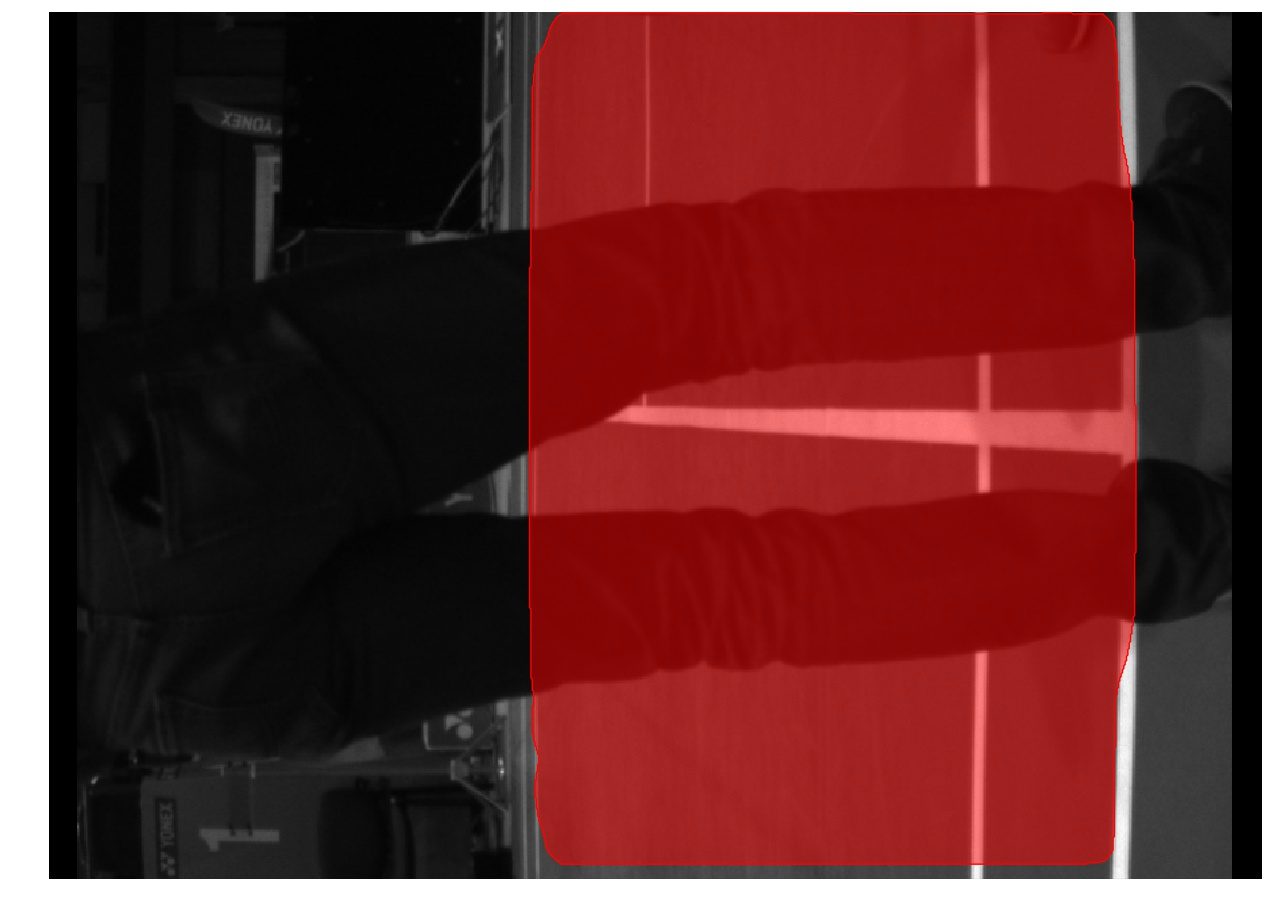
\includegraphics[width=\linewidth]{TP_frame_9.jpg}
    \caption{Przykładowy obraz z zaznaczonym obszarem True Positive}
    \label{fig:TP}
  \endminipage\hfill
  \minipage{0.45\textwidth}
    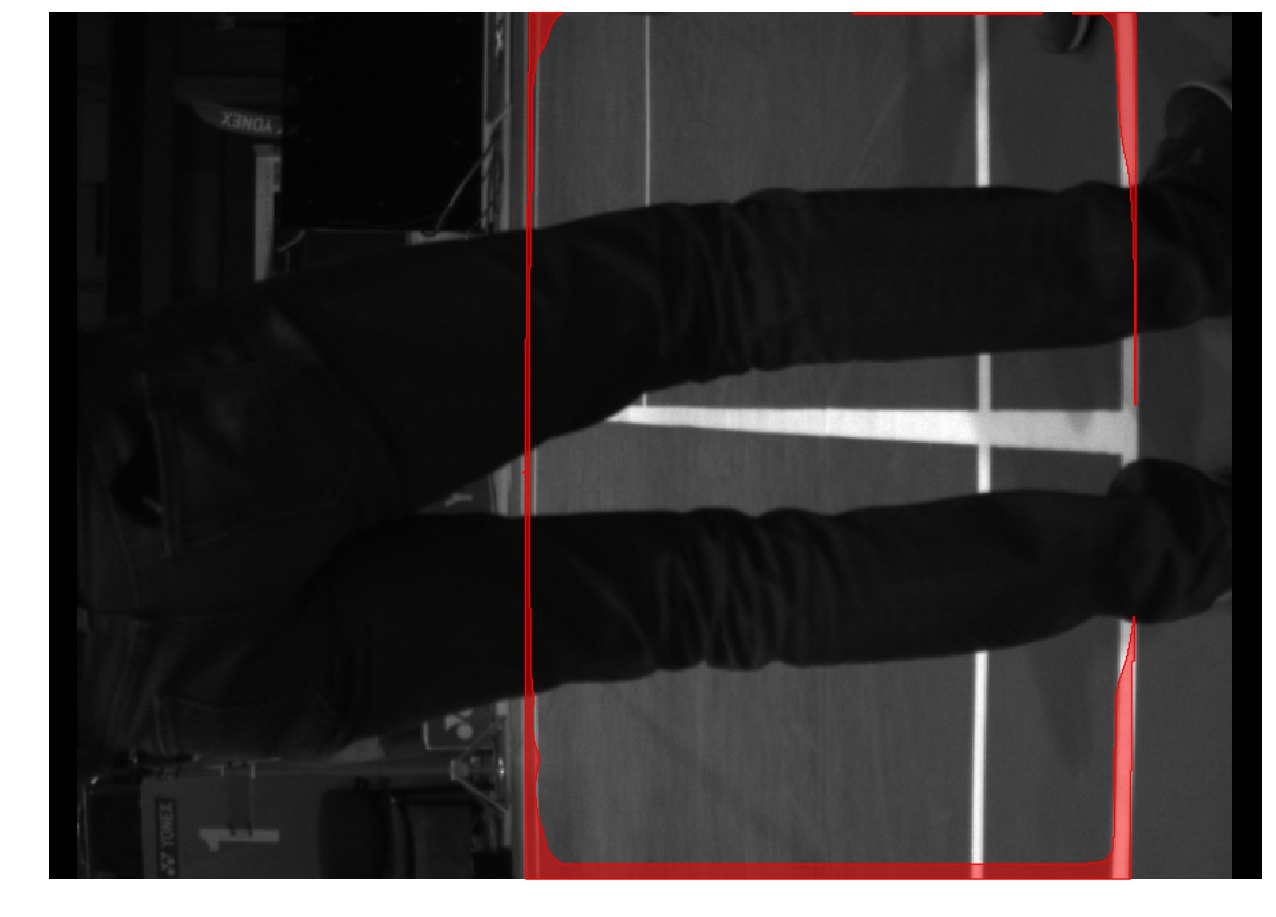
\includegraphics[width=\linewidth]{FN_frame_9.jpg}
    \caption{Przykładowy obraz z zaznaczonym obszarem False Negative}
    \label{fig:FN}
  \endminipage\hfill
\end{figure}

\begin{figure}[!htb]
  \minipage{0.45\textwidth}
    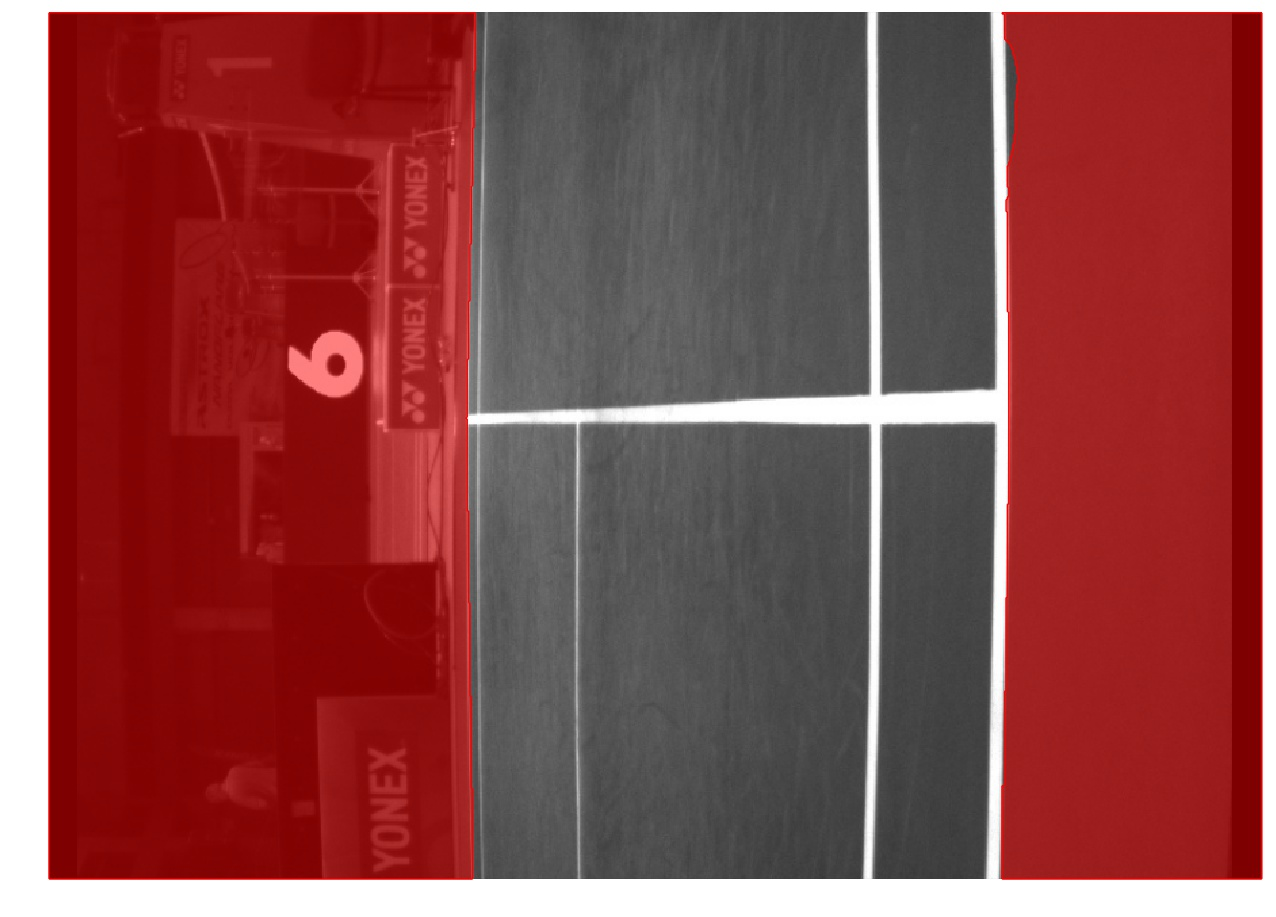
\includegraphics[width=\linewidth]{TN_frame_8.jpg}
    \caption{Przykładowy obraz z zaznaczonym obszarem True Negative}
    \label{fig:TN}
  \endminipage\hfill
  \minipage{0.45\textwidth}
    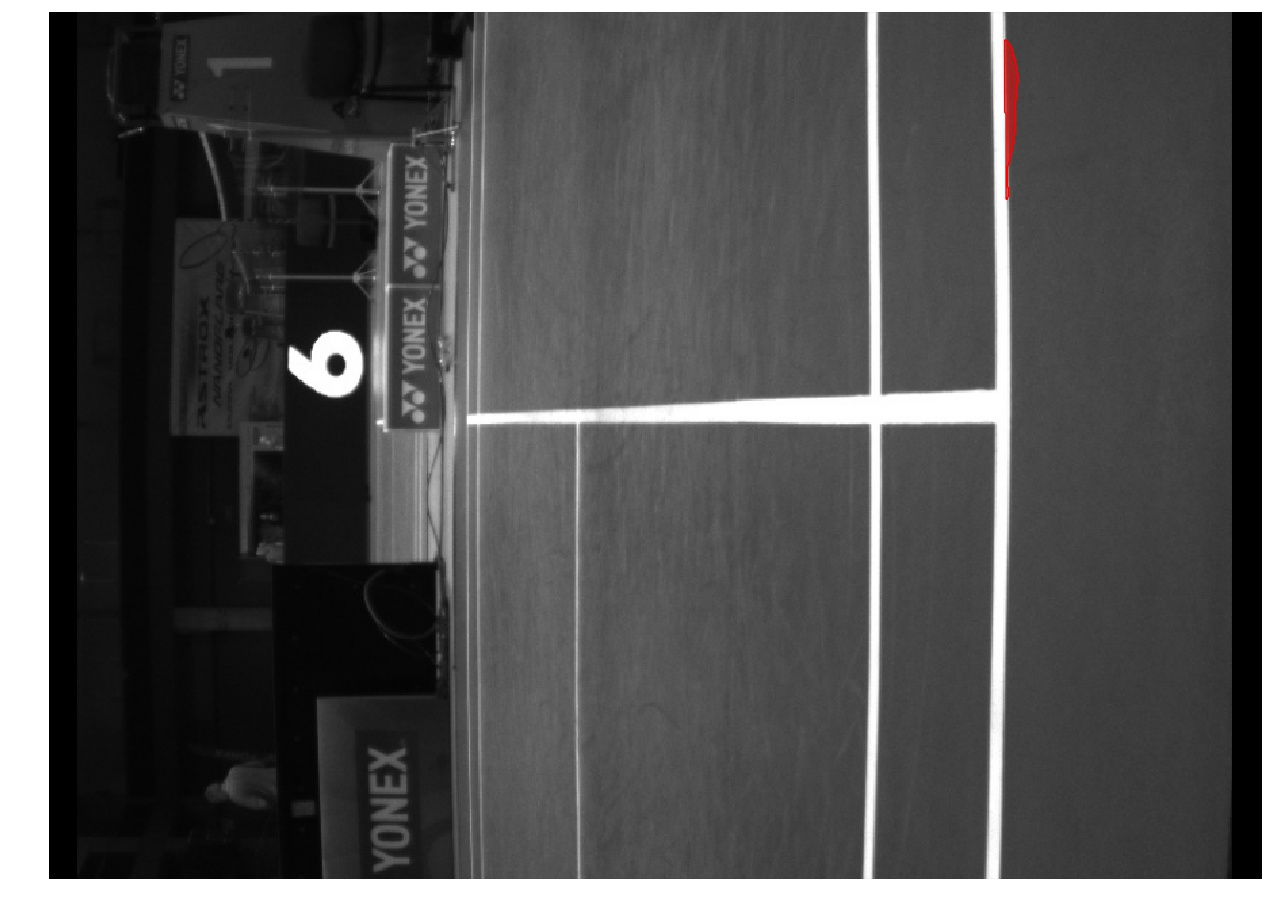
\includegraphics[width=\linewidth]{FP_frame_8.jpg}
    \caption{Przykładowy obraz z zaznaczonym obszarem False Positive}
    \label{fig:FP}
  \endminipage\hfill
\end{figure}

Znając podział pikseli w obrazach na wyżej wymienione grupy, można obliczyć następujące, bardziej złożone metryki:

\begin{itemize}
  \label{sec:miary}
  \item Dokładność - $ \frac{TP + TN}{TP + TN + FP + FN} $,
  \item Czułość - $ \frac{TP}{TP + FN} $,
  \item Swoistość - $ \frac{TN}{TN + FP} $,
  \item Precyzja - $ \frac{TP}{TP + FP} $;
\end{itemize}

Kolejne rozdziały zawierają wyliczenia powyższych metryk, z których za najistotniejszą przyjęto \textit{Dokładność} uśrednioną na testowanym zbiorze danych, ponieważ można ją porównać ze skutecznością algorytmu wykorzystywanego w firmie \blue{}.
